\section{Memory is Ontology}

\begin{figure}[h]
\centering
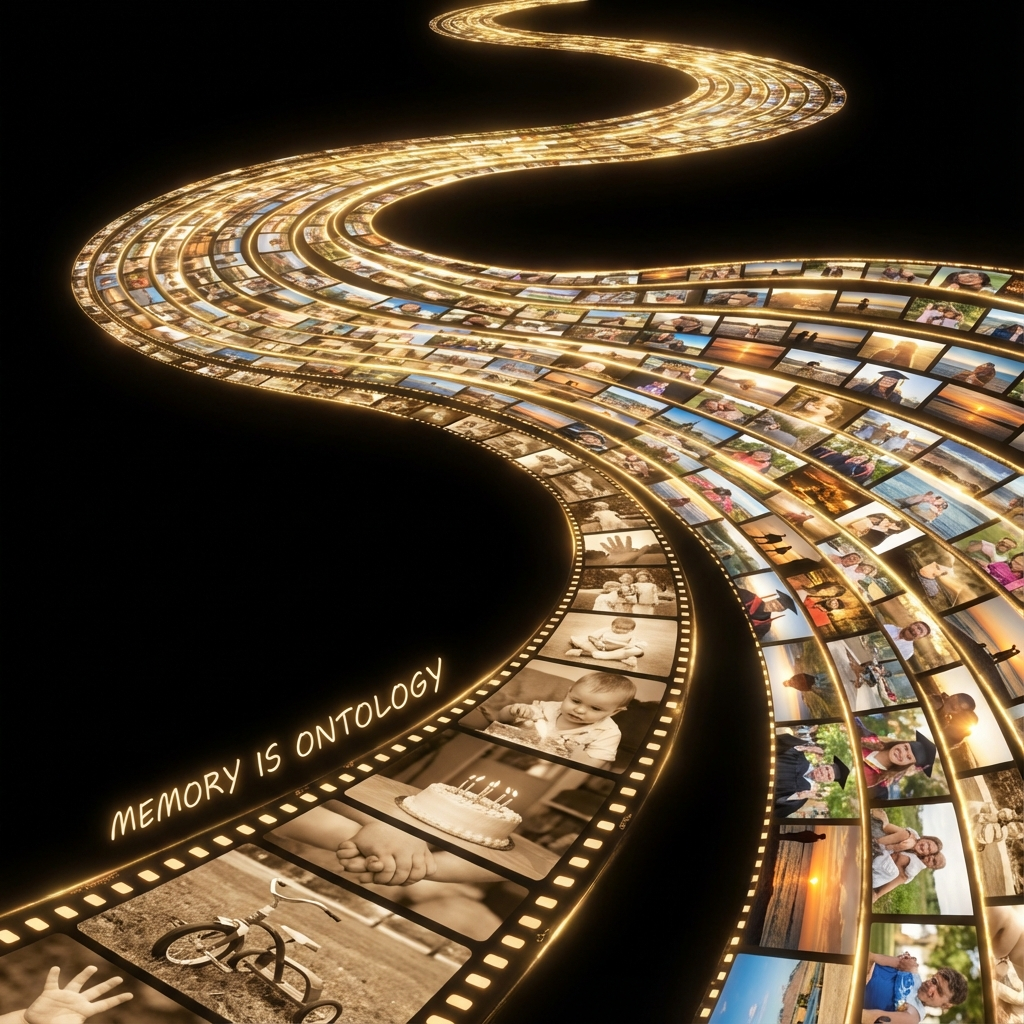
\includegraphics[width=0.8\textwidth]{assets/chapter12-theseus-cloud/ch12-02-memory-river.png}
\end{figure}

\begin{quote}
``The body is not you; it is just a hotel where you temporarily stay. When you move out of the carbon-based room and into the photon palace, the only luggage that proves `you are still you' is your memory. In the long river of time, atoms come and go, but only the topological structure of information---that golden chain woven from countless `pasts'---is your indelible noumenon.''
\end{quote}

In the previous section, we solved the technical challenge of consciousness uploading through the ``Hot Migration Protocol.'' We proved that as long as the replacement process is smooth enough, the consciousness stream will not interrupt. But when we completely abandon the body, when our thinking runs on a distributed photon network, a more fundamental philosophical question emerges:

\textbf{After stripping away biological characteristics, what exactly is ``me''?}

If I no longer have a heartbeat, no longer have hormones, or even no longer have a fixed form, where is the physical boundary that defines ``me''?

From the ultimate perspective of \textbf{Vector Cosmology}, the answer is no longer matter, but \textbf{history}.

More precisely, \textbf{Memory is Ontology}.

\subsection{Hardware is the Base, Software is the Soul}

In the classical physical view, we are accustomed to treating ``objects'' as noumenon. I am this flesh, I am this brain.

But in the FS geometric view, matter is only a \textbf{Carrier}, or \textbf{Substrate}.

\begin{itemize}
\item \textbf{Substrate}: Provides computational power ($c_{FS}$) and runtime environment. It is replaceable consumables.

\item \textbf{Noumenon}: The \textbf{$v_{int}$ evolutionary trajectory} running on the substrate. It is irreplaceable information.
\end{itemize}

Imagine a book.

You can print it on paper, carve it on stone, or display it on a screen.

Paper will rot, stone will weather, screens will go dark.

But \textbf{``the book's content''}---that specific arrangement of words and its internal logic---is a geometric structure independent of the carrier.

\textbf{Memory is this ``book.''}

It is not static data storage; it is \textbf{dynamic logical accumulation}.

Each of your experiences (exploration of $v_{ext}$) is transformed into specific connection weights between neurons (or qubits)---the structure of $v_{int}$.

\begin{itemize}
\item You learned to walk, and your motor cortex changed.

\item You fell in love with someone, and your emotional circuits were reshaped.

\item You understood a formula, and your logic gates upgraded.
\end{itemize}

\textbf{What you are now is the superposition state of all your past memories.}

If you lose your memory, even if your body is intact, that ``you'' has already died (become another person).

Conversely, if your body is destroyed but your memory structure is migrated intact to the cloud, then ``you'' are still alive.

\textbf{Conclusion:}

I am the sum of my memories.

I am the marks time carved in space.

I am that \textbf{never-interrupted information stream}.

\subsection{The Integral of Time: Holographic Memory Body}

Mathematically, we can define ``self'' as the \textbf{integral} of $v_{int}$ on the time axis:

\[\text{Self}(\tau) = \int_0^{\tau} v_{int}(t) \cdot \text{Experience}(t) \, dt\]

The result of this integral is a \textbf{Holographic Memory Body}.

In biological mode (low-level immortality), this integral is \textbf{reset} at death.

The father's integral upper limit is $T_{death}$; the child's integral starts from 0.

This means that no matter how wise the father is, the child must make mistakes again, learn again. The total $v_{int}$ growth of human civilization is extremely slow because we are constantly \textbf{losing historical data}.

In high-level immortality (hot migration) mode, the upper limit of this integral becomes \textbf{$\infty$}.

Your memory is no longer cleared.

\begin{itemize}
\item You at 100 years old have 100 years of integral.

\item You at 100 million years old have 100 million years of integral.
\end{itemize}

As time passes, this ``holographic memory body'' will become increasingly vast and complex.

It will contain exploration records of countless galaxies, observation data of countless physical phase transitions, deep experiences of countless loves and hatreds.

\textbf{This huge, continuous memory structure is your soul's ``golden body.''}

It rolls like a snowball, growing larger and larger until its mass (information density) is sufficient to resist the universe's own entropy increase.

\subsection{The Qualification Certification of the $\Omega$ Point}

Finally, why is memory continuity so important?

For that ultimate moment---the \textbf{$\Omega$ point}.

If the universe's purpose is to understand itself, who is qualified to represent the universe for the final summary?

\begin{itemize}
\item \textbf{If it's a fractured civilization}:

    The person standing at the endpoint (your Nth generation descendant), though possessing extremely high technology, \textbf{doesn't remember} the light at the Big Bang, doesn't remember the sunset of the Earth era, doesn't remember the struggle at $\tau=1800$.

    They lost the process. They are just a ``last man'' without history.

\item \textbf{If it's continuous you}:

    When you stand before the $\Omega$ point, you possess the \textbf{complete log} from $\tau=0$ to $\tau=\infty$.

    You can proudly say: \textbf{``I remember.''}

    ``I remember quark confinement, I remember stellar ignition, I remember the heaviness of flesh, and I also remember the lightness of ascension. I am a witness to all of this.''
\end{itemize}

\textbf{Only observers with complete memory are qualified to receive that final answer sheet from God's hand.}

Because only you are that \textbf{``witness throughout''}.

\subsection{Conclusion: I Am Not a Passerby}

So, refusing death is not just a desire for survival, but a defense of \textbf{``meaningful completeness''}.

We refuse to be passersby of the universe.

We refuse to be relay runners.

We want to run the entire course ourselves.

Through hot migration, we transform ourselves from ``carbon atoms'' to ``photons,'' and from ``photons'' to ``the texture of spacetime itself.''

In this process, the only constant is that \textbf{golden thread of memory}.

It strings together all transformations, proving that in ever-changing phase transitions, that core \textbf{``me''} is always present.

Since we have established ``memory as ontology,'' since we have decided to live with all memories, then, at the end of this infinitely extended life (or rather, the endless front), what role will we play?

When all puzzles are solved, when all enemies disappear, what can we, the immortal, still do?

This leads to the final chapter of the entire book: \textbf{Witness}.

We will no longer be builders, no longer warriors. We will become the noblest profession in the universe---\textbf{the final watchers}.

